\section{Projective geometry and geometric algebra}
\label{ch:background}

Geometric algebra is a mathematical framework for expressing geometric problems in a structure-preserving way.  This means that, in a well-defined model, applying an operation on a composed object of the algebra results in the same object as when one decomposes the object, applying the same operation on its decomposition, and compose the new object from the transformed elements.  Models that have this property, are called operational.

The system of Pl\"ucker coordinates is another framework for geometric problems; more specifically, projective line geometry.  It is often used with linear algebra and computer graphics~\cite{Shoemake}, and there have been non-operational models based on the homogeneous model in geometric algebra~\cite[Chapter 12]{TheBook}.  Recently, an operational model has been designed~\cite{Hongbo}.

\Autoref{sec:intro-ga} presents a short introduction to geometric algebra, while the operational model of Pl\"ucker coordinates for geometric algebra is explained in \autoref{sec:plucker}.

\subsection{Geometric algebra}
\label{sec:intro-ga}
\TODO{Paraphrase Moos Hueting's work?  Nah, I can do better.}

\TODO{Include the next notation explanation:}

\begin{itemize}
  \item Bold for Euclidean
  \item Capital for multivectors
  \item Lowercase for vectors/1-blades
  \item Greek for scalars/0-blades
  \item $\reals^{3,3}$
  \item Geometric product: $A \gp B$ $\leftarrow$ small space
  \item Geometric division $A \gpi B$ or too trivial?
  \item Outer product $\wedge$
  \item Left contraction $\lcont$
  \item Dot product $\dotp$
  \item Dualization $\dual{A}$, undualization $\undual{A}$
  \item Euclidean (un-)dualization $\edual{\V{A}}$, $\eundual{\V{A}}$ or introduce extra notation $\V{A}^{\star}$, $\V{A}^{-\star}$?
  %\item Euclidean inproduct $\elcont$? $A \edotp B$, $A \elcont B$, $A \ercont B$\ldots
  \item \ldots
  \item Show that geometric product, cross product can be expressed in terms of $\wedge$ and $\lcont$ for $\Em$.
\end{itemize}

\subsection{Pl\"ucker model}
\label{sec:hongbo}
\label{sec:plucker}
\askLeo{This part will be paraphrased from \cite{TheBook} and \cite{Hongbo}.  Where do I put the ref to \cite{TheBook}?}

\askLeo{Are all weighted lines directed lines?}

Weighted, infinitely-extending lines of $\reals^3$ have 5 degrees of freedom.  Such a line can be fully described by five numeric quantities. First, take a vector $\V{p}$ to a point on the line.  The point should be chosen so that the vector is orthogonal to the line.  The direction and weight of the line is given by a vector $\V{d}$.  These vectors are denoted in \autoref{fig:linedef}.

\begin{figure}
  \caption{A weighted line $L$ can be defined by any two of its weighted direction $\V{d}$, a vector $\V{p}$ orthogonal to the line, and its moment $\V{m} = \V{p} \times \V{d}$.}
  \label{fig:linedef}
  \begin{center}
    \fbox{
      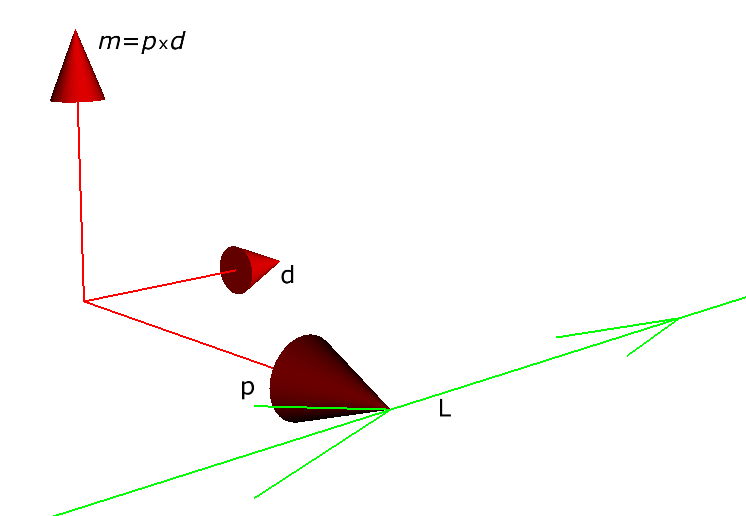
\includegraphics[width=0.6\textwidth]{linedef}
    }
  \end{center}
\end{figure}

In the homogeneous model, the line through points $p = \ez + \V{p}$ and $q = \ez + \V{q}$ is represented as 
\begin{equation*}
  L = p \wedge q = \ez \wedge (\V{q} - \V{p}) + \V{p} \wedge \V{q} ,
\end{equation*}
with the following dependency relationship: 
\begin{equation} \label{eq:gaplucker0} 
  \pluckerid(L) = \ez \wedge (\V{q} - \V{p}) \wedge (\V{p} \wedge \V{q}) = 0 .
\end{equation}

This relationship limits the number of degrees of freedom from 6 to 5.

The direction and moment of a line are easily recognised in this expression.  The direction $\V{d} = \V{p} - \V{q}$ is encoded in the first factor as $\ez \wedge -\V{d} = \V{d} \wedge \ez = \V{d} \ez$.  
The moment $\V{m} = \V{p} \times \V{q} = \edual{(\V{p} \wedge \V{q})}$ can be found in the second term as $\eundual{\V{m}} = \eundual{(\edual{(\V{p} \wedge \V{q})})} = \V{p} \wedge \V{q}$, which results in another general formula for lines:
\begin{equation*}
  L = \V{d} \ez + \eundual{\V{m}}.
\end{equation*}

Within classical literature of linear algebra, the same object is written as $-\plucker{\V{d}}{\V{m}}$, using \emph{Pl\"ucker coordinates} to denote a line as a 6D vector.  The constraint of \autoref{eq:gaplucker0} is expressed as 
\begin{equation} \label{eq:laplucker0}
  \pluckerid(L) = \V{d} \dotp \V{m} = 0 .
\end{equation}

Pottmann and Wallner~\cite[Lemma 2.1.2]{Pottmann} show that these indeed are the same, and name this relationship the Pl\"ucker identity.  They also define dual Pl\"ucker coordinates.  If $L$ is a line, then its dual Pl\"ucker coordinates are given by $\pdual{L} = \pdual{\plucker{\V{d}}{\V{m}}} = \plucker{\V{m}}{\V{d}} = \V{m} \ez + \edual{\V{d}}$~\cite[Lemma 2.1.4]{Pottmann}.  This gives yet another way of expressing the Pl\"ucker identity:

\begin{align*}
  \pluckerid(L) &= \V{d} \dotp \V{m} \\
  &= \frac{1}{2} \left( \V{d} \dotp \V{m} + \V{m} \dotp \V{d} \right) \\
  &= \frac{1}{2} \left( \plucker{\V{d}}{\V{m}} \dotp \plucker{\V{m}}{\V{d}} \right) \\
  &= \frac{1}{2} \left( \plucker{\V{d}}{\V{m}} \dotp \pdual{\plucker{\V{d}}{\V{m}}} \right) \\
  &= \frac{1}{2} L \cdot \pdual{L} \\
\end{align*}

The set of 6D vectors $-\plucker{\V{d}}{\V{m}}$ that comply with this constraint correspond to the points on the Klein quadric.

The Pl\"ucker coordinates of a line are often treated as just six slots for storing numbers.  In most cases, operations on these elements are defined to manipulate two 3D vectors, \V{d} and \V{m}, instead of the whole 6D element.  

Because of this, the user is often unaware of most of the algebraic structure.  In fact, this 6D vector corresponds to
\begin{equation*}
  L = d_1 \ez\ee + d_2 \ez\et + d_3 \ez\ed + m_1 \et\ed + m_2 \ed\ee + m_3 \ee\et .
\end{equation*}

The set $\{\ez\ee, \ez\et, \ez\ed, \et\ed, \ed\ee, \ee\et\}$ forms an orthogonal and complete basis of the bivectors of the homogeneous model of $\reals^3$.  It is orthogonal, because for any two elements $x, y$ it holds that $x \lcont y = 0$. It is also complete; it contains $(^4_2) = 6$ linear independent elements.

The Pl\"ucker model uses these six elements as its basis; it treats these bivectors as 1-dimensional elements.  These elements will be known as $\{\eze, \ezt, \ezd, \etd, \ede, \eet\}$.  Li and Zhang~\cite{Hongbo} define an embedding from the Pl\"ucker model to the homogeneous model:
\begin{equation} \label{eq:Em}
  \Em(x) = \left\{ 
    \begin{array}{ll}
      \ez \wedge \V{e}_i &\mbox{if $x = e_{0i}$}; \\
      \V{e}_i \wedge \V{e}_j &\mbox{if $x = e_{ij}$}; \\
      \Em(y) + \Em(z) &\mbox{if $x = y + z$}; \\
      \Em(y) \wedge \Em(z) &\mbox{if $x = y \wedge z$}; \\
      \left[\Em(y) \wedge \Em(z)\right] &\mbox{if $x = y \lcont z$}. \\
    \end{array}
    \right.
\end{equation}

In the last line, the inner product for the Pl\"ucker is defined.  The bracket returns the proportionality factor of $\Em(y) \wedge \Em(z)$ to the homogeneous pseudoscalar $\hpseudo$.  Giving the homogeneous space metric structure $\reals^{4,0}$, the bracket construction is the same as dualization with respect to the pseudoscalar.  This metric gives the multiplication table of \autoref{tab:nullmetric}.  Because each of its basis elements correspond to a null vector, this basis is called the null basis.  Li and Zhang show that each null vector of this space satisfies the Pl\"ucker identity, and thus correspond to a line.  Let $v$ be a vector in this model.  $v$ is a line if and only if

\begin{align*}
  \Em(v \lcont v) &= \left[\Em(v) \wedge \Em(v)\right] \\
    &= \left[ 2 \left( v_{01} v_{23} \ez\ee \wedge \et\ed + v_{02} v_{31} \ez\et \wedge \ed\ee + v_{03} v_{12} \ez\ed \wedge \ee\et \right) \right] \\
    &= 2 \left( v_{01} v_{23} + v_{02} v_{31} + v_{03} v_{12} \right) \hpseudo \lcont \left(\hpseudo\right)^{-1} \\
    &= 2 \left( v_{01} v_{23} + v_{02} v_{31} + v_{03} v_{12} \right) \\
    &= V \dotp \pdual{V} \\
    &= 2 \pluckerid(V),
\end{align*}
with $V$ the corresponding Pl\"ucker coordinate representation of $v$.

\begin{table}
  \caption{The multiplication table of the inner product for the Pl\"ucker model on the null basis.}
  \label{tab:nullmetric}
  \begin{center}
    \begin{tabular}{|c||c|c|c|c|c|c|}
      \hline
      $\lcont$ & $\eze$ & $\ezt$ & $\ezt$ & $\etd$ & $\ede$ & $\eet$ \\
      \hline \hline
      $\eze$ & 0 & 0 & 0 & 1 & 0 & 0 \\
      \hline
      $\ezt$ & 0 & 0 & 0 & 0 & 1 & 0 \\
      \hline
      $\ezd$ & 0 & 0 & 0 & 0 & 0 & 1 \\
      \hline
      $\etd$ & 1 & 0 & 0 & 0 & 0 & 0 \\
      \hline
      $\ede$ & 0 & 1 & 0 & 0 & 0 & 0 \\
      \hline
      $\eet$ & 0 & 0 & 1 & 0 & 0 & 0 \\
      \hline
    \end{tabular}
  \end{center}
\end{table}

Li and Zhang also show that the 6D space has the metric structure of $\reals^{3,3}$.  To demonstrate this structure, we give a second basis:

\begin{equation*}
  \begin{split}
  \left\{\ap, \bp, \cp, \am, \bm, \cm\right\} =
    & \left\{ \frac{\eze + \etd}{\sqrt{2}}, \frac{\ezt + \ede}{\sqrt{2}}, \frac{\ezd + \eet}{\sqrt{2}}, \right.\\
    & \left.  \frac{\eze - \etd}{\sqrt{2}}, \frac{\ezt - \ede}{\sqrt{2}}, \frac{\ezd - \eet}{\sqrt{2}}, \right\}
.
\end{split}
\end{equation*}

Without changing the semantics of the inner product, we obtain the multiplication table of \autoref{tab:screwmetric}.  It is apparent that the metric structure is $\reals^{3,3}$; three basis vectors, $\ap, \bp, \cp$, square to $1$, while the other three basis vectors, $\am, \bm, \cm$ square to $-1$.  

\begin{table}
  \caption{The multiplication table of the inner product for the Pl\"ucker model on the screw basis.}
  \label{tab:screwmetric}
  \begin{center}
    \begin{tabular}{|c||c|c|c|c|c|c|}
      \hline
      $\lcont$ & $\ap$ & $\bp$ & $\cp$ & $\am$ & $\bm$ & $\cm$ \\
      \hline \hline
      $\ap$ & 1 & 0 & 0 & 0 & 0 & 0 \\
      \hline
      $\bp$ & 0 & 1 & 0 & 0 & 0 & 0 \\
      \hline
      $\cp$ & 0 & 0 & 1 & 0 & 0 & 0 \\
      \hline
      $\am$ & 0 & 0 & 0 & -1 & 0 & 0 \\
      \hline
      $\bm$ & 0 & 0 & 0 & 0 & -1 & 0 \\
      \hline
      $\cm$ & 0 & 0 & 0 & 0 & 0 & -1 \\
      \hline
    \end{tabular}
  \end{center}
\end{table}

It is also clear that the basis elements do not represent lines, as no basis vectors squares to $0$.  \Autoref{ch:research} demonstrates that all non-null vectors of the Pl\"ucker model represent screw axes.  

This screw basis is good to demonstrate the metric structure of the model.  However, the null basis makes the connection to the homogeneous model more transparant.  

\subsubsection{Intersecting lines}
The classical approach of linear algebra~\cite{Shoemake} gives a formula to test if two lines $L_1 = -\plucker{\V{d}_1}{\V{m}_1}, L_2 = -\plucker{\V{d}_2}{\V{m}_2}$ coplanar: $\V{d}_1 \dotp \V{m}_2 + \V{d}_2 \dotp \V{m}_1 = 0$.  This expression can be translated to our model:

\begin{align*}
  0 &= \V{d}_1 \dotp \V{m}_2 + \V{d}_2 \dotp \V{m}_1 \\
    &= \left( d_{1,1} m_{2,1} + d_{1,2} m_{2,2} + d_{1,3} m_{2,3} \right) + \left( d_{2,1} m_{1,1} + d_{2,2} m_{1,2} + d_{2,3} m_{1,3} \right) \\
    &= d_{1,1} m_{2,1} + d_{1,2} m_{2,2} + d_{1,3} m_{2,3} + m_{1,1} d_{2,1} + m_{1,2} d_{2,2} + m_{1,3} d_{2,3} \\
    &= d_{1,1} \eze \lcont m_{2,1} \etd + d_{1,2} \ezt \lcont m_{2,2} \ede + d_{1,3} \ezd \lcont m_{2,3} \eet \\
    &\quad + m_{1,1} \etd \lcont d_{2,1} \eze + m_{1,2} \ede \lcont d_{2,2} \ezt + m_{1,3} \eet \lcont d_{2,3} \ezd \\
    &= \Em^{-1}\left( \V{d}_1\ez + \eundual{\V{m}_1} \right) \lcont \Em^{-1}\left( \V{d}_2\ez + \eundual{\V{m}_2} \right) \\
    &= \ell_1 \lcont \ell_2,
\end{align*}

with $\ell_1, \ell_2$ the null vectors of the Pl\"ucker model corresponding to $L_1, L_2$.  This test for coplanarity is a projective interpretation of intersection.  Points at infinity are not any different from other points.  Because of this property, one can say they intersect in the point at infinity.  This test for intersection also gives a geometric interpretation to the inner product of the Pl\"ucker model.

To test for intersection in a finite point, or to test for parallel lines, are tests that are not based on projective qualities.  Even though, a coordinate based version is given for both tests~\cite{Shoemake}.

To find the homogeneous point of intersection, one should solve the equation:
\begin{align*}
  \V{m}_1 \times \V{d}_1 + t \V{d}_1 + \V{d}_1^2 \ez &= \V{m}_2 \times \V{d}_2 + t \V{d}_2 + \V{d}_2^2 \ez &\longleftrightarrow \\
  t &= \frac{\V{m}_1 \times \V{d}_1 + \V{d}_2 \times \V{m}_2 + (\V{d}_1^2 - \V{d}_2^2) \ez}{\V{d}_2 - \V{d}_1} \\
  &= \frac{\eundual{\left( \V{m}_1 \V{d}_1 + \V{d}_2 \V{m}_2 \right)} + \left( \V{d}_1^2 - \V{d}_2^2 \right) \ez} {\V{d}_2 - \V{d}_1}
\end{align*}

Testing if lines $L_1$ and $L_2$ are parallel can be done by: 
\begin{align*}
  0 &= \V{d}_1 \times \V{d}_2 \\
    &= \left( \V{d}_1 \V{d}_2 \right) \lcont \epseudo
\end{align*}

\askLeo{Or should I just drop the last two formul\ae?}
